\section*{Background}
\label{sec:synopsis:background}
The dissertation addresses the long-standing goal in artificial intelligence of enabling machines to understand and answer human questions using large collections of structured knowledge. Knowledge Graphs (KGs) are well-suited for this, offering interconnected facts for precise answers. The advent of Large Language Models (LLMs) has significantly impacted this field, as LLMs possess strong language understanding and generation capabilities, along with a substantial amount of implicitly stored factual knowledge. However, using LLMs for Knowledge Graph Question Answering (KGQA) presents challenges, notably the issue of ``hallucination''---generating plausible but incorrect answers~\cite{lin-etal-2022-truthfulqa, DBLP:conf/emnlp/RobertsRS20, DBLP:journals/csur/JiLFYSXIBMF23, DBLP:journals/corr/abs-2401-01313}---and the lack of transparency in their reasoning, making factual verification difficult.

As LLMs become more prevalent, KGs gain further importance as reliable sources of explicit, structured knowledge. While LLMs excel at text generation and semantic understanding, they struggle with rapidly changing facts and integrating new information without corrupting existing knowledge. For instance, LLMs alone often fail on comparative questions without access to structured data, as shown in work on the CAM 2.0 system~\cite{DBLP:conf/coling/ShalloufHSVMPBN24}. Research detailed in the dissertation~\cite{pletenev-etal-2025-much} explored the problems of adding new facts into LLMs using Low-rank Adaptation (LoRA), showing that such additions can be harmful, potentially degrading general QA performance if new knowledge is domain-specific, leading to overrepresentation and reduced ability to express uncertainty. These limitations underscore the critical need for robust methods to synergistically combine LLM textual abilities with KG factual grounding, rather than solely attempting to update LLM parametric knowledge. This dissertation focuses on developing and evaluating novel methods for such effective LLM-KG integration to enhance the accuracy and trustworthiness of KGQA systems.

\section*{Relevance of the Work}
\label{sec:synopsis:relevance}
The relevance of this work stems from the pressing need to improve the reliability and factual accuracy of question answering systems in an era increasingly dominated by LLMs. While LLMs offer unprecedented capabilities in natural language understanding and generation, their propensity for generating incorrect information (hallucinations) and their opaque reasoning processes are significant barriers to their deployment in critical applications. Knowledge Graphs, as vast repositories of structured, verifiable facts, offer a powerful complementary resource. This dissertation is relevant because it directly tackles the challenge of effectively fusing these two technologies. By developing methods that leverage KGs to ground LLM outputs, constrain answer generation, and provide verifiable evidence, the work aims to create KGQA systems that are not only more accurate but also more trustworthy and interpretable. The practical significance lies in enabling more dependable AI systems for information access, while the theoretical relevance lies in advancing our understanding of how symbolic knowledge representation and sub-symbolic deep learning models can be productively combined. The development of new datasets like ShortPathQA~\cite{DBLP:conf/nldb/SalnikovSPQA25} further stimulates community research in this vital area.

\section*{Dissertation Objectives}
\label{sec:synopsis:objectives}
This dissertation aims to develop and empirically evaluate novel methods for combining Large Language Models (LLMs) with Knowledge Graphs (KGs) to create Question Answering (QA) systems that are more accurate, dependable, and controllable. The primary objectives are:
\begin{itemize}
    \item To enhance answer candidate generation in KGQA by leveraging the semantic understanding capabilities of LLMs in conjunction with explicit type constraints derived from KGs. This includes the development of the Answer Candidate Type (ACT) Selection method, which predicts the likely semantic type of an answer and uses this to filter and refine candidate answers (detailed in Chapter~3).
    \item To facilitate controllable and standardized community research on the fusion of KGs and LLMs for KGQA, through the development and public release of the \texttt{ShortPathQA} dataset~\cite{DBLP:conf/nldb/SalnikovSPQA25}. This resource provides pre-computed KG subgraphs, allowing researchers to concentrate on fusion methodologies rather than complex KG processing tasks (introduced in Chapter~4).
    \item To improve the factual correctness and controllability of LLM-generated answers by developing a system to re-rank candidate answers using structural proof derived from KG subgraphs. This involves identifying relevant subgraphs connecting question entities to LLM-generated candidates, extracting diverse features from these subgraphs, and employing various ranking models to select candidates with stronger KG-based evidence (detailed in Chapter~4).
\end{itemize}

\section*{Scientific Novelty}
\label{sec:synopsis:novelty}
The scientific novelty of this dissertation lies in the development and evaluation of innovative methods for integrating LLMs and KGs to address key challenges in KGQA:
\begin{enumerate}
    \item \textbf{Novel Answer Candidate Typing and Selection:} The Answer Candidate Type (ACT) Selection method (Chapter~3, \cite{DBLP:journals/corr/abs-2310-07008}) introduces a new approach to KGQA by uniquely combining an LLM's ability to predict the semantic type of an answer with explicit type information from a KG (e.g., Wikidata's P31 `instance of' property). This type-based validation of LLM-generated candidates acts as a powerful filter and scoring mechanism, significantly improving candidate quality, even when the LLM initially errs on the fact but correctly identifies the type.
    \item \textbf{Controllable Fusion via Subgraph Reranking:} The dissertation proposes a novel framework (Chapter~4, \cite{DBLP:journals/corr/abs-2310-02166}) for enhancing the factuality of LLM outputs by reranking answer candidates based on structural evidence from KG subgraphs. The novelty encompasses:
    \begin{itemize}
        \item The systematic extraction of relevant KG subgraphs connecting question entities to multiple LLM-generated answer candidates.
        \item Comprehensive feature engineering from these subgraphs, including graph-theoretic metrics (e.g., PageRank, Katz centrality), textual features, and various Graph2Text (G2T) sequence representations (Deterministic, T5-based, GAP-based).
        \item The application and comparative analysis of diverse ranking models (from regression to neural rankers like MPNet) to utilize these multi-modal subgraph features for promoting factually grounded answers.
    \end{itemize}
    \item \textbf{Creation of a Specialized Evaluation Resource (ShortPathQA):} The development and publication of the \texttt{ShortPathQA} dataset (Chapter~4, \cite{DBLP:conf/nldb/SalnikovSPQA25}) is a significant novel contribution. This dataset directly supports research on Controllable Fusion via Subgraph Reranking and aims to foster community exploration. As the first QA resource offering pre-computed KG subgraphs, \texttt{ShortPathQA} enables researchers to focus on subgraph reasoning and reranking, isolated from upstream complexities, facilitating targeted evaluation of controllable fusion techniques.
\end{enumerate}

\section*{Theoretical and Practical Significance}
\label{sec:synopsis:significance}
The research presented in this dissertation holds both theoretical and practical significance for Natural Language Processing and Artificial Intelligence, particularly in KGQA.

Theoretically, this work contributes to a deeper understanding of how the complementary strengths of LLMs (semantic understanding, fluency) and KGs (structured factual knowledge, verifiability) can be synergistically combined. It explores specific fusion mechanisms beyond simple retrieval augmentation, towards nuanced candidate refinement and evidence-based reranking. The investigation into type-based filtering (ACT Selection) illuminates the implicit semantic knowledge in LLMs and its explicit leveraging with KG schema. The study of subgraph-based reranking contributes to theories of evidence-based reasoning in QA, showing how KG structural path information can signal factuality and control LLM outputs. The \texttt{ShortPathQA} dataset~\cite{DBLP:conf/nldb/SalnikovSPQA25} facilitates more focused theoretical explorations into subgraph reasoning.

Practically, the developed methodologies, ACT Selection~\cite{DBLP:journals/corr/abs-2310-07008} and subgraph-based reranking~\cite{DBLP:journals/corr/abs-2310-02166}, offer pathways to improve QA system accuracy and reliability, crucial for real-world applications where misinformation is costly. By grounding LLM outputs in verifiable KG facts, this research aids in building more trustworthy AI. Subgraph analysis enhances interpretability by allowing answers to be traced to KG evidence. ACT Selection offers a resource-efficient strategy to boost smaller LLMs, making high-quality KGQA more accessible. The \texttt{ShortPathQA} dataset~\cite{DBLP:conf/nldb/SalnikovSPQA25} lowers the entry barrier for developing and evaluating LLM-KG fusion techniques. System demonstrations (Chapter~5), including APIs and visualization tools, provide tangible proofs-of-concept and reusable components for advanced KGQA applications.

\section*{Research Methodology}
\label{sec:synopsis:methodology}
The research in this dissertation employs a multifaceted methodology combining theoretical development with empirical experimentation and system implementation:
\begin{enumerate}
    \item \textbf{Literature Review and Problem Formulation (Chapter~2):} A comprehensive review of existing research in KGQA, LLMs, and LLM-KG fusion strategies (e.g.,~\cite{DBLP:journals/tkde/PanLWCWW24, DBLP:conf/ijcai/0001LW0S0Y24}) identified research gaps and formulated precise research questions.
    \item \textbf{Method Development - ACT Selection (Chapter~3):} Based on observing LLM behavior regarding answer type prediction, a pipeline was designed. This pipeline generates initial answer candidates using LLMs (e.g., T5, BART with Diverse Beam Search~\cite{DBLP:journals/corr/VijayakumarCSSL16-diverse-beam-search}), employs multilingual entity linking (e.g., mGENRE~\cite{decao2021multilingual}) to connect entities to Wikidata, infers the expected answer type using the LLM and aggregates type information from KG \texttt{instance-of} relations, and ranks candidates using a weighted scoring mechanism (type scores, KG neighborhood scores, LLM generation scores, and question-property similarity using Sentence-BERT~\cite{reimers-2019-sentence-bert}).
    \item \textbf{Method Development - Controllable Fusion via Subgraph Reranking (Chapter~4):} Hypothesizing that KG path-based evidence can improve LLM answer factuality, a reranking pipeline was designed. This generates multiple answer candidates (Diverse Beam Search), extracts KG subgraphs (shortest paths from Wikidata), engineers diverse features (graph features: PageRank~\cite{page1999pagerank}, Katz centrality~\cite{katz1953new}, etc.; text features with MPNet~\cite{DBLP:conf/nips/Song0QLL20}), and compares reranking models (semantic, regression, CatBoost~\cite{DBLP:conf/nips/ProkhorenkovaGV18-catboost}, neural MPNet).
    \item \textbf{Dataset Creation (ShortPathQA - Chapter~4, \cite{DBLP:conf/nldb/SalnikovSPQA25}):} To address the need for a focused benchmark, questions from Mintaka~\cite{DBLP:conf/coling/SenAS22-mintaka} and new complex questions were collected. LLM-generated candidates and unified shortest path subgraphs from Wikidata were compiled and published.
    \item \textbf{Experimental Evaluation:} Utilized established KGQA datasets (SQWD~\cite{SQ_WD}, RuBQ~\cite{korablinov2020rubq}, Mintaka~\cite{DBLP:conf/coling/SenAS22-mintaka}) and \texttt{ShortPathQA}~\cite{DBLP:conf/nldb/SalnikovSPQA25}. Fine-tuned LLMs (T5, BART, spaCy NER). Employed appropriate metrics (Hits@1, Hits@N, F1-score). Conducted ablation studies and error analysis. Compared against baselines including standalone LLMs (e.g., ChatGPT) and KGQA systems (e.g., QAnswer~\cite{diefenbach2020towards}, KEQA~\cite{Huang2019KnowledgeGE}).
    \item \textbf{System Implementation and Demonstration (Chapter~5):} Developed practical system pipelines (baseline Seq2Seq, M3M~\cite{DBLP:conf/acl/RazzhigaevSMBP23}, ACT Selection) using Python, FastAPI, PyTorch, HuggingFace Transformers, spaCy. Created a subgraph visualization tool (HTML, JavaScript, D3.js).
\end{enumerate}

\section*{Validation of the Research Results, Reliability}
\label{sec:synopsis:validation}
The research findings are validated through rigorous empirical evaluation on multiple standard benchmark datasets and newly created resources, ensuring reliability via:
\begin{itemize}
    \item \textbf{Standardized Datasets and Metrics:} ACT Selection (Chapter~3) was evaluated on SQWD~\cite{SQ_WD}, RuBQ~\cite{korablinov2020rubq} (English translations), and a subset of Mintaka~\cite{DBLP:conf/coling/SenAS22-mintaka} (one-hop English questions) using Hits@1. Controllable fusion methods (Chapter~4) used Mintaka (excluding count and yes/no questions) and the newly introduced ShortPathQA dataset~\cite{DBLP:conf/nldb/SalnikovSPQA25}. Evaluation metrics included Hits@N (N=1, 2, 3) and F1-score.
    \item \textbf{Comparison with Baselines:} Performance was compared against base Text-to-Text models (T5, BART), specialized KGQA systems (e.g., QAnswer~\cite{diefenbach2020towards}, KEQA~\cite{Huang2019KnowledgeGE}), large conversational models (ChatGPT), initial LLM predictions (T5-Large-SSM, T5-XL-SSM, Mistral, Mixtral), and for ShortPathQA, zero-shot LLMs (GPT-4o, LLaMA3-8b-Instruct) and supervised models (MPNet, fine-tuned LLaMA3-8b-Instruct).
    \item \textbf{Ablation Studies:} Comprehensive ablation studies assessed individual contributions of different components (e.g., scoring mechanisms in ACT Selection, feature types in controllable fusion).
    \item \textbf{Error Analysis:} Qualitative error analysis provided deeper insights (e.g., ACT Selection demonstrated 94\% correct answer type prediction for T5-Large-SSM on SQWD, up from 61\%; G2T analysis highlighted T5's superior factual accuracy over GAP).
    \item \textbf{Cross-Model and Cross-Dataset Evaluation:} Methods were evaluated across different LLM architectures and sizes (T5, BART, Mistral, Mixtral) and multiple datasets, demonstrating robustness.
    \item \textbf{Reproducibility:} Publication of code (e.g., M3M pipeline~\cite{DBLP:conf/acl/RazzhigaevSMBP23}, ShortPathQA dataset and code~\cite{DBLP:conf/nldb/SalnikovSPQA25}) and detailed experimental setups support reproducibility. ShortPathQA's manual test set curation involved multiple annotators, achieving high agreement (Cohen's kappa 0.81 for question type, avg. quality 4.81/5).
\end{itemize}
These measures collectively ensure conclusions are well-supported by empirical evidence and proposed methods offer reliable KGQA improvements.

\section*{Approbation of the Work and Publications}
\label{sec:synopsis:approbation}
The research presented in this dissertation has been disseminated through peer-reviewed publications in international conferences and journals, and through participation in shared tasks and system demonstrations. The key contributions have been presented to and validated by the scientific community.
The publications by the author that form the basis of or are related to this dissertation are:
\begin{enumerate}
    \item Anton Razzhigaev*, \textbf{Mikhail Salnikov*}, Valentin Malykh, Pavel Braslavski, and Alexander Panchenko. 2023. A System for Answering Simple Questions in Multiple Languages. In Proceedings of the 61st Annual Meeting of the Association for Computational Linguistics (Volume 3: System Demonstrations), pages 524–537, Toronto, Canada. Association for Computational Linguistics. CORE A*
    \item \textbf{Mikhail Salnikov}, Maria Lysyuk, Pavel Braslavski, Anton Razzhigaev, Valentin A. Malykh, and Alexander Panchenko. 2023. Answer Candidate Type Selection: Text-To-Text Language Model for Closed Book Question Answering Meets Knowledge Graphs. In Proceedings of the 19th Conference on Natural Language Processing (KONVENS 2023), pages 155–164, Ingolstadt, Germany. Association for Computational Linguistics. 
    \item \textbf{Mikhail Salnikov}, Hai Le, Prateek Rajput, Irina Nikishina, Pavel Braslavski, Valentin Malykh, and Alexander Panchenko. 2023. Large Language Models Meet Knowledge Graphs to Answer Factoid Questions. In Proceedings of the 37th Pacific Asia Conference on Language, Information and Computation, pages 635–644, Hong Kong, China. Association for Computational Linguistics. CORE C.
    \item Andrey Sakhovskiy*, \textbf{Mikhail Salnikov*}, Irina Nikishina, Aida Usmanova, Angelie Kraft, Cedric Möller, Debayan Banerjee, Junbo Huang, Longquan Jiang, Rana Abdullah, Xi Yan, Dmitry Ustalov, Elena Tutubalina, Ricardo Usbeck, and Alexander Panchenko. 2024. TextGraphs 2024 Shared Task on Text-Graph Representations for Knowledge Graph Question Answering. In Proceedings of TextGraphs-17: Graph-based Methods for Natural Language Processing, pages 116–125, Bangkok, Thailand. Association for Computational Linguistics.
    \item \textbf{Mikhail Salnikov*}, Andrey Sakhovskiy*, Irina Nikishina, Aida Usmanova, Angelie Kraft, Cedric Möller, Debayan Banerjee, Junbo Huang, Longquan Jiang, Rana Abdullah, Xi Yan, Elena Tutubalina, Ricardo Usbeck, and Alexander Panchenko. (2025). ShortPathQA: A Dataset for Controllable Fusion of Large Language Models with Knowledge Graphs. In \textit{Natural Language Processing and Information Systems - 30th International Conference on Applications of Natural Language to Information Systems, NLDB 2025}. Workshop on CORE A* Conference.
    \item Ahmad Shallouf*, Hanna Herasimchyk*, \textbf{Mikhail Salnikov*}, Rudy Alexandro Garrido Veliz*, Natia Mestvirishvili*, Alexander Panchenko, Chris Biemann, and Irina Nikishina. 2024. CAM 2.0: End-to-End Open Domain Comparative Question Answering System. In Proceedings of the 2024 Joint International Conference on Computational Linguistics, Language Resources and Evaluation (LREC-COLING 2024), pages 2657–2672, Torino, Italia. ELRA and ICCL. CORE B.
    \item Maria Lysyuk, \textbf{Mikhail Salnikov}, Pavel Braslavski, and Alexander Panchenko. (2024). Konstruktor: A Strong Baseline for Simple Knowledge Graph Question Answering In International Conference on Applications of Natural Language to Information Systems, pp. 107-118. Cham: Springer Nature Switzerland, 2024. CORE C.
    \item Dmitrii Iarosh, Alexander Panchenko, and \textbf{Mikhail Salnikov}. (2025). On Reducing Factual Hallucinations in Graph-to-Text Generation Using Large Language Models. In \textit{Proceedings of the Workshop on Generative AI and Knowledge Graphs (GenAIK)}.
    \item Sergey Pletenev, Maria Marina, Daniil Moskovskiy, Vasily Konovalov, Pavel Braslavski, Alexander Panchenko, and \textbf{Mikhail Salnikov}. 2025. How Much Knowledge Can You Pack into a LoRA Adapter without Harming LLM?. In Findings of the Association for Computational Linguistics: NAACL 2025, pages 4309–4322, Albuquerque, New Mexico. Association for Computational Linguistics. CORE A.
\end{enumerate}
(* denotes shared first authorship)

\section*{Author's Contribution}
\label{sec:synopsis:contribution}
Author's personal contribution to the research presented in this dissertation is as follows:
\begin{itemize}
    \item \textbf{ACT Selection Method Development (publication 2):} The author was fully responsible for the conceptualization, implementation, and experimental validation of the Answer Candidate Type Selection pipeline, including the design of the four-component scoring mechanism.
    \item \textbf{Subgraph Reranking Framework and supported research (publication 3, 4, 8, 9):} The author led the full development of the controllable fusion methodology and the design of the experiments. The implementation and experimental design for the Graph-To-Text (G2T) models were developed by the author's advisor with significant contributions from Hai Le, Dmitrii Iarosh, and Ivan Lazichny. Olga Tsymboi and Egor Cheremiskin implemented experiments with the Mistral and Mixtral models.
    \item \textbf{ShortPathQA Dataset Creation (publication 5):} The author had full responsibility for the dataset design and the subgraph generation pipeline. The annotation framework and question curation for the manual portion of the dataset were handled by Andrey Sakhovskiy and Irina Nikishina. Andrey Sakhovskiy conducted experiments with encoder-only baselines.
    \item \textbf{System Demonstration Creation (publication 1, 6, 7):} The author had full responsibility for creating the system demonstrations. Dmitrii Iarosh assisted with the development of the subgraph visualization tool and related DevOps tasks.
\end{itemize}

\section*{The Structure and Volume of the Dissertation}
\label{sec:synopsis:structure}
The dissertation is structured into five main chapters, preceded by an introduction and followed by a conclusion, encompassing a comprehensive exploration of the research topic.
The dissertation comprises an Introduction, which sets out the problem, objectives, and contributions. Chapter 2 provides a review of background concepts and related work in KGQA, LLMs, and their fusion. Chapter 3 details the Answer Candidate Type (ACT) Selection methodology. Chapter 4 presents the framework for controllable fusion of LLMs and KGs using subgraph reranking, and introduces the ShortPathQA dataset. Chapter 5 describes the system demonstrations and implementations of the developed methods. The work concludes by summarizing key findings and outlining future research directions. The dissertation also includes a list of references and may contain appendices with supplementary material.

\section*{Contents of the Dissertation}
\label{sec:synopsis:contents}
This dissertation presents a cohesive body of research focused on enhancing Knowledge Graph Question Answering (KGQA) by synergistically integrating Large Language Models (LLMs) with Knowledge Graphs (KGs). A key contribution, detailed in Chapter 3, is the development of the Answer Candidate Type (ACT) Selection method~\cite{DBLP:journals/corr/abs-2310-07008}. This approach innovatively refines LLM-generated answer candidates by leveraging the observation that LLMs often correctly predict an answer's semantic type even when factually erring. The work involved designing and implementing a novel pipeline that generates initial candidates using LLMs with Diverse Beam Search, performs multilingual entity linking (mGENRE~\cite{decao2021multilingual}) to ground entities in Wikidata, infers the expected answer type by combining LLM predictions with KG type information (such as Wikidata's `instance of' P31 property), and then ranks all candidates using a weighted scoring mechanism. This mechanism incorporates type agreement, KG neighborhood presence, original LLM generation scores, and question-property similarity (calculated using Sentence-BERT~\cite{reimers-2019-sentence-bert}). The ACT Selection method demonstrated significant improvements in Hits@1 accuracy on benchmark datasets (SQWD, RuBQ, Mintaka one-hop) and showed that it can make smaller LLMs competitive with much larger ones, offering a resource-efficient way to enhance KGQA performance. Selected results are shown in Table~\ref{tab:act_selection:comparsion_hits1_sqwd}.

\begin{table}[htb]
\caption{Comparsion of the ACT Selection with KGQA baselines in terms of Hits@1 for SimpleQuestion-Wikidata (SQWD) with T5-Large-ssm fine-tuned on its training part and T5-11b-ssm-nq in zero-shot mode. (Table from Chapter 3 of the dissertation)}
\label{tab:act_selection:comparsion_hits1_sqwd}
\centering
    \begin{tabular}{lcc}
    \hline
    Model & SQWD & RuBQ en \\
    \hline
    QAnswer & 33.31 & 32.30 \\
    KEQA TransE PTBG & \textbf{48.89} & 33.80 \\
    % MEKER TransE PTBQ & 53.50 & 49.50 \\
    ChatGPT & 15.32 & 36.53 \\ \hline
    T5-Large-ssm (fine-tuned) & 23.66 & 21.44 \\ 
    \text{Ours}: T5-Large-ssm (fine-tuned) & 47.42 & 26.02 \\ \hline 
    T5-11b-ssm-nq (zero-shot) & 10.94 & 33.38 \\
    \text{Ours}: T5-11b-ssm-nq (zero-shot) & 38.51 & \textbf{38.31} \\
    \hline
    \end{tabular}
\end{table}

Further advancing the fusion of LLMs and KGs, the dissertation, primarily in Chapter 4, introduces a novel framework for controllable KG-LLM fusion via subgraph reranking~\cite{DBLP:journals/corr/abs-2310-02166}. This methodology aims to improve the factuality and controllability of LLM outputs by re-evaluating candidate answers based on structural evidence from KG subgraphs. The general pipeline for this fusion strategy is illustrated in Figure~\ref{fig:synopsis:fusion_pipeline}.

\begin{figure}[htb]
    \centering
    \includegraphics[width=0.9\columnwidth]{new_paper_big_pipeline.pdf}
    \caption{The proposed method for reranking language model answers with KGs. The method includes subgraph extraction, feature extraction, and various ranker approaches (Figure from Chapter 4 of the dissertation).}
    \label{fig:synopsis:fusion_pipeline}
\end{figure}

A core component of this framework is \textbf{subgraph extraction}, detailed in Section 4.2 of the dissertation. This process is crucial for isolating the most relevant portion of the vast KG for a given question-answer pair. For each pair, the subgraph extraction algorithm first identifies all shortest paths within the KG (Wikidata in this research) connecting the entities mentioned in the question to a specific LLM-generated answer candidate. Once these shortest paths are found, an induced subgraph is constructed. This means taking all unique nodes (entities) present in these paths and including all existing edges (relationships) from the original KG that connect any two nodes within this set. This results in a compact, focused graph structure that contains the primary entities and the most direct relational evidence connecting them. This targeted subgraph, rather than the entire KG, is then used for the subsequent feature engineering and reranking steps, making the process more efficient and the evidence more pertinent.

The overall work involved developing a pipeline that systematically extracts these KG subgraphs. Following extraction, comprehensive feature engineering was performed, creating features categorized into graph-theoretic metrics (e.g., PageRank~\cite{page1999pagerank}, Katz centrality~\cite{katz1953new}), textual features (question-answer concatenations encoded via MPNet~\cite{DBLP:conf/nips/Song0QLL20}), and three distinct types of Graph2Text (G2T) sequence representations (Deterministic, T5-based~\cite{DBLP:journals/corr/abs-2007-08426}, and GAP-based~\cite{DBLP:conf/coling/ColasAW22-GAP}). These rich, multi-modal features were then used to train and evaluate diverse reranking models, ranging from simpler regression models and CatBoost~\cite{DBLP:conf/nips/ProkhorenkovaGV18-catboost} to more complex neural rankers like MPNet, effectively promoting answers with stronger KG-based proof. This reranking framework consistently improved Hits@N scores on the Mintaka dataset. The selected results are shown in Table~\ref{tab:controllable_fusion:features_importance}.

\begin{table}[htbp]
    \caption{Hits@1 performance of different feature sets (Text, Graph, and Graph2Text variants) across various reranking models (Linear Regression, Logistic Regression, CatBoost, and MPNet). Results are shown for different answer source models (T5-Large-SSM, T5-XL-SSM, Mistral, and Mixtral). All models were fine-tuned on the Mintaka training set using identical hyperparameters. The dash (--) indicates that the feature type is not applicable for the given model. (Table from Chapter 4 of the dissertation)}
    \label{tab:controllable_fusion:features_importance}
        \resizebox{\textwidth}{!}{
            \begin{tabular}{c|l|c|c|c|c}
            \toprule
            \textbf{\makecell{Answers\\Source}}                & \textbf{Features} & \textbf{\makecell{Linear\\Regression}} & \textbf{\makecell{Logistic\\Regression}} & \textbf{CatBoost}     & \textbf{MPNet}        \\
            \midrule
            \multirow{5}{*}{\textbf{\begin{turn}{45}\makecell{T5-Large\\SSM}\end{turn}}} & Text & 0,2695 & 0,2605 & 0,2458 & 0,2620 \\ 
                                            & Graph & 0,2338 & 0,2335 & 0,1935 & -- \\ 
                                            & Graph2Text (Determ Lin) & 0,2550 & 0,2440 & 0,2405 & 0,3398 \\ 
                                            & Graph2Text (T5) & 0,2505 & 0,2313 & 0,2398 & 0,3493 \\ 
                                            & Graph2Text (GAP) & 0,2393 & 0,2925 & 0,2395 & 0,3395 \\ \hline
            \multirow{5}{*}{\textbf{\begin{turn}{45}\makecell{T5-XL\\SSM}\end{turn}}} & Text & 0,2955 & 0,2850 & 0,2593 & 0,3418 \\ 
                                            & Graph & 0,2550 & 0,2613 & 0,2760 & -- \\ 
                                            & Graph2Text (Determ Lin) & 0,2640 & 0,2598 & 0,2580 & 0,3923 \\ 
                                            & Graph2Text (T5) & 0,2593 & 0,2538 & 0,2485 & 0,3905 \\ 
                                            & Graph2Text (GAP) & 0,2563 & 0,2503 & 0,2590 & 0,3573 \\ \hline
            \multirow{5}{*}{\textbf{\begin{turn}{45}Mistral\end{turn}}} & Text & 0,4760 & 0,4730 & 0,3917 & 0,5115 \\ 
                                            & Graph & 0,3575 & 0,3558 & 0,3632 & -- \\ 
                                            & Graph2Text (Determ Lin) & 0,3960 & 0,3970 & 0,3862 & 0,5007 \\ 
                                            & Graph2Text (T5) & 0,4013 & 0,3985 & 0,4012 & 0,4965 \\ 
                                            & Graph2Text (GAP) & 0,3885 & 0,3850 & 0,3787 & 0,4917 \\ \hline
            \multirow{5}{*}{\textbf{\begin{turn}{45}Mixtral\end{turn}}} & Text & 0,4883 & 0,4853 & 0,4040 & 0,5237 \\ 
                                            & Graph & 0,3698 & 0,3680 & 0,3755 & -- \\ 
                                            & Graph2Text (Determ Lin) & 0,4083 & 0,4093 & 0,3985 & 0,5130 \\ 
                                            & Graph2Text (T5) & 0,4135 & 0,4108 & 0,3940 & 0,5087 \\ 
                                            & Graph2Text (GAP) & 0,4008 & 0,3973 & 0,3910 & 0,5040 \\ 
            \bottomrule
            \end{tabular}%
        }
    \end{table}

To facilitate research in this area and address the engineering challenges of KG processing, the dissertation also presents the \texttt{ShortPathQA} dataset~\cite{DBLP:conf/nldb/SalnikovSPQA25}, a significant contribution detailed in Chapter 4. This novel benchmark is the first to provide pre-computed KG subgraphs (from Wikidata) alongside questions (from Mintaka~\cite{DBLP:conf/coling/SenAS22-mintaka} and new manual curations) and LLM-generated answer candidates. By offering this resource, the work lowers the barrier for entry for researchers focusing on LLM-KG fusion and reranking techniques, allowing for standardized and reproducible experimentation without the overhead of large-scale KG hosting and subgraph retrieval. The utility of \texttt{ShortPathQA} was demonstrated through comprehensive baseline evaluations.

Finally, the practical applicability and translation of these research contributions into functional systems are demonstrated in Chapter 5. This chapter details the design and implementation of several key software artifacts. These include: a baseline Seq2Seq pipeline (T5-based) for initial answer generation; the M3M pipeline~\cite{DBLP:conf/acl/RazzhigaevSMBP23}, an earlier multilingual KGQA system developed by the author and colleagues that showcases advanced KG interaction and semantic matching; a deployable version of the ACT Selection pipeline (from Chapter 3); and an interactive subgraph visualization tool. This tool, built with web technologies (HTML, JavaScript, D3.js) and a FastAPI backend, allows users to explore KG subgraphs and their G2T verbalizations, directly supporting the research on controllable fusion (from Chapter 4). These implemented systems, with source code made available, serve as tangible proofs-of-concept for the dissertation's methodologies and offer valuable, reusable tools and APIs for the research community, effectively bridging theoretical advancements with practical KGQA solutions. The system demonstration interface is shown in Figure~\ref{fig:synopsis:m3m_demo}.

\begin{figure}[htb]
    \centering
    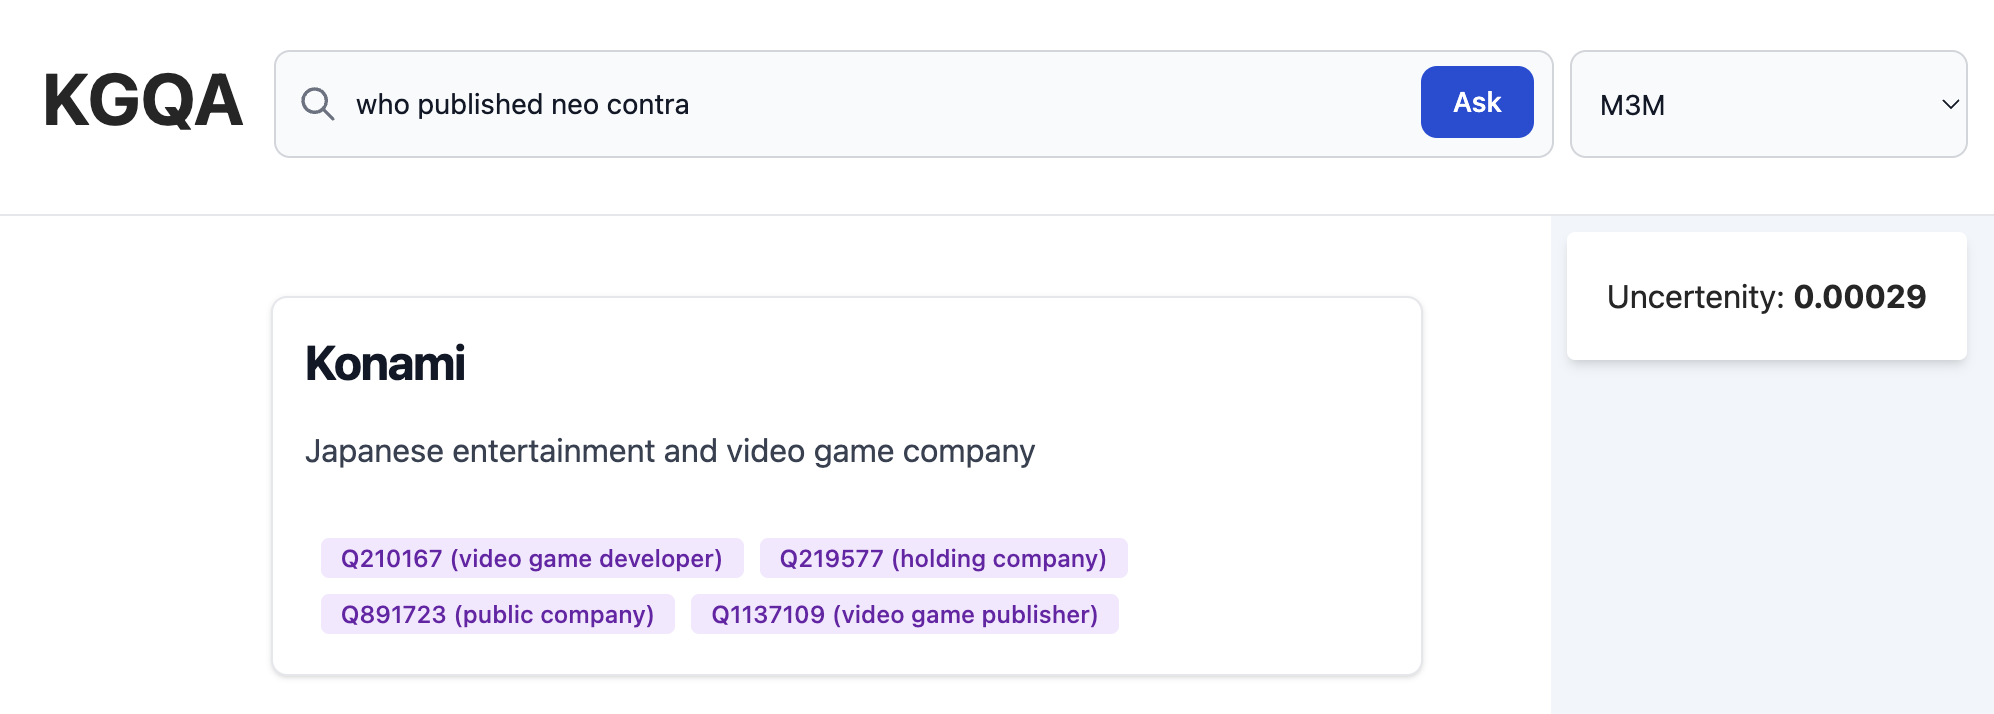
\includegraphics[width=0.8\columnwidth]{demo_m3m.png}
    \caption{The developed system demonstration interface with example for question-answers for M3M pipeline. (Figure from Chapter 5 of the dissertation).}
    \label{fig:synopsis:m3m_demo}
\end{figure}


\section*{Conclusion}
\label{sec:synopsis:conclusion}
This dissertation has systematically addressed critical challenges in Knowledge Graph Question Answering (KGQA) by developing and evaluating novel methods for the synergistic fusion of Large Language Models (LLMs) and Knowledge Graphs (KGs). The research successfully achieved its objectives of enhancing answer accuracy, reliability, and controllability.

The core contributions include: (1) The Answer Candidate Type (ACT) Selection method~\cite{DBLP:journals/corr/abs-2310-07008}, which leverages LLM semantic type understanding and KG type constraints to significantly refine answer candidates, proving effective even for smaller LLMs. (2) A comprehensive framework for Controllable Fusion via Subgraph Reranking~\cite{DBLP:journals/corr/abs-2310-02166}, where LLM-generated answers are re-evaluated based on structural evidence from KG subgraphs, utilizing diverse feature engineering and robust ranking models. (3) The creation and release of the \texttt{ShortPathQA} dataset~\cite{DBLP:conf/nldb/SalnikovSPQA25}, a novel resource with pre-computed subgraphs that facilitates focused research on LLM-KG fusion mechanisms.

Through rigorous experimentation on established benchmarks (SQWD~\cite{SQ_WD}, RuBQ~\cite{korablinov2020rubq}, Mintaka~\cite{DBLP:conf/coling/SenAS22-mintaka}) and the new \texttt{ShortPathQA} dataset, the proposed methods demonstrated marked improvements over baseline LLM performance and traditional KGQA approaches. The practical utility of these methods was further showcased through the implementation of several system demonstrations~\cite{DBLP:conf/acl/RazzhigaevSMBP23}, including interactive tools.

The findings underscore the significant potential of combining the strengths of LLMs and KGs. Future work may explore extensions to more complex reasoning tasks, broader multilingual applications, and further refinements in knowledge integration and explainability. This research lays a strong foundation for building more intelligent, trustworthy, and factually grounded AI systems capable of effectively utilizing vast stores of both unstructured text and structured knowledge.
